% Options for packages loaded elsewhere
\PassOptionsToPackage{unicode}{hyperref}
\PassOptionsToPackage{hyphens}{url}
%
\documentclass[
]{book}
\usepackage{amsmath,amssymb}
\usepackage{lmodern}
\usepackage{iftex}
\ifPDFTeX
  \usepackage[T1]{fontenc}
  \usepackage[utf8]{inputenc}
  \usepackage{textcomp} % provide euro and other symbols
\else % if luatex or xetex
  \usepackage{unicode-math}
  \defaultfontfeatures{Scale=MatchLowercase}
  \defaultfontfeatures[\rmfamily]{Ligatures=TeX,Scale=1}
\fi
% Use upquote if available, for straight quotes in verbatim environments
\IfFileExists{upquote.sty}{\usepackage{upquote}}{}
\IfFileExists{microtype.sty}{% use microtype if available
  \usepackage[]{microtype}
  \UseMicrotypeSet[protrusion]{basicmath} % disable protrusion for tt fonts
}{}
\makeatletter
\@ifundefined{KOMAClassName}{% if non-KOMA class
  \IfFileExists{parskip.sty}{%
    \usepackage{parskip}
  }{% else
    \setlength{\parindent}{0pt}
    \setlength{\parskip}{6pt plus 2pt minus 1pt}}
}{% if KOMA class
  \KOMAoptions{parskip=half}}
\makeatother
\usepackage{xcolor}
\usepackage{color}
\usepackage{fancyvrb}
\newcommand{\VerbBar}{|}
\newcommand{\VERB}{\Verb[commandchars=\\\{\}]}
\DefineVerbatimEnvironment{Highlighting}{Verbatim}{commandchars=\\\{\}}
% Add ',fontsize=\small' for more characters per line
\usepackage{framed}
\definecolor{shadecolor}{RGB}{248,248,248}
\newenvironment{Shaded}{\begin{snugshade}}{\end{snugshade}}
\newcommand{\AlertTok}[1]{\textcolor[rgb]{0.94,0.16,0.16}{#1}}
\newcommand{\AnnotationTok}[1]{\textcolor[rgb]{0.56,0.35,0.01}{\textbf{\textit{#1}}}}
\newcommand{\AttributeTok}[1]{\textcolor[rgb]{0.77,0.63,0.00}{#1}}
\newcommand{\BaseNTok}[1]{\textcolor[rgb]{0.00,0.00,0.81}{#1}}
\newcommand{\BuiltInTok}[1]{#1}
\newcommand{\CharTok}[1]{\textcolor[rgb]{0.31,0.60,0.02}{#1}}
\newcommand{\CommentTok}[1]{\textcolor[rgb]{0.56,0.35,0.01}{\textit{#1}}}
\newcommand{\CommentVarTok}[1]{\textcolor[rgb]{0.56,0.35,0.01}{\textbf{\textit{#1}}}}
\newcommand{\ConstantTok}[1]{\textcolor[rgb]{0.00,0.00,0.00}{#1}}
\newcommand{\ControlFlowTok}[1]{\textcolor[rgb]{0.13,0.29,0.53}{\textbf{#1}}}
\newcommand{\DataTypeTok}[1]{\textcolor[rgb]{0.13,0.29,0.53}{#1}}
\newcommand{\DecValTok}[1]{\textcolor[rgb]{0.00,0.00,0.81}{#1}}
\newcommand{\DocumentationTok}[1]{\textcolor[rgb]{0.56,0.35,0.01}{\textbf{\textit{#1}}}}
\newcommand{\ErrorTok}[1]{\textcolor[rgb]{0.64,0.00,0.00}{\textbf{#1}}}
\newcommand{\ExtensionTok}[1]{#1}
\newcommand{\FloatTok}[1]{\textcolor[rgb]{0.00,0.00,0.81}{#1}}
\newcommand{\FunctionTok}[1]{\textcolor[rgb]{0.00,0.00,0.00}{#1}}
\newcommand{\ImportTok}[1]{#1}
\newcommand{\InformationTok}[1]{\textcolor[rgb]{0.56,0.35,0.01}{\textbf{\textit{#1}}}}
\newcommand{\KeywordTok}[1]{\textcolor[rgb]{0.13,0.29,0.53}{\textbf{#1}}}
\newcommand{\NormalTok}[1]{#1}
\newcommand{\OperatorTok}[1]{\textcolor[rgb]{0.81,0.36,0.00}{\textbf{#1}}}
\newcommand{\OtherTok}[1]{\textcolor[rgb]{0.56,0.35,0.01}{#1}}
\newcommand{\PreprocessorTok}[1]{\textcolor[rgb]{0.56,0.35,0.01}{\textit{#1}}}
\newcommand{\RegionMarkerTok}[1]{#1}
\newcommand{\SpecialCharTok}[1]{\textcolor[rgb]{0.00,0.00,0.00}{#1}}
\newcommand{\SpecialStringTok}[1]{\textcolor[rgb]{0.31,0.60,0.02}{#1}}
\newcommand{\StringTok}[1]{\textcolor[rgb]{0.31,0.60,0.02}{#1}}
\newcommand{\VariableTok}[1]{\textcolor[rgb]{0.00,0.00,0.00}{#1}}
\newcommand{\VerbatimStringTok}[1]{\textcolor[rgb]{0.31,0.60,0.02}{#1}}
\newcommand{\WarningTok}[1]{\textcolor[rgb]{0.56,0.35,0.01}{\textbf{\textit{#1}}}}
\usepackage{longtable,booktabs,array}
\usepackage{calc} % for calculating minipage widths
% Correct order of tables after \paragraph or \subparagraph
\usepackage{etoolbox}
\makeatletter
\patchcmd\longtable{\par}{\if@noskipsec\mbox{}\fi\par}{}{}
\makeatother
% Allow footnotes in longtable head/foot
\IfFileExists{footnotehyper.sty}{\usepackage{footnotehyper}}{\usepackage{footnote}}
\makesavenoteenv{longtable}
\usepackage{graphicx}
\makeatletter
\def\maxwidth{\ifdim\Gin@nat@width>\linewidth\linewidth\else\Gin@nat@width\fi}
\def\maxheight{\ifdim\Gin@nat@height>\textheight\textheight\else\Gin@nat@height\fi}
\makeatother
% Scale images if necessary, so that they will not overflow the page
% margins by default, and it is still possible to overwrite the defaults
% using explicit options in \includegraphics[width, height, ...]{}
\setkeys{Gin}{width=\maxwidth,height=\maxheight,keepaspectratio}
% Set default figure placement to htbp
\makeatletter
\def\fps@figure{htbp}
\makeatother
\setlength{\emergencystretch}{3em} % prevent overfull lines
\providecommand{\tightlist}{%
  \setlength{\itemsep}{0pt}\setlength{\parskip}{0pt}}
\setcounter{secnumdepth}{5}
\usepackage{booktabs}
\ifLuaTeX
  \usepackage{selnolig}  % disable illegal ligatures
\fi
\usepackage[]{natbib}
\bibliographystyle{plainnat}
\IfFileExists{bookmark.sty}{\usepackage{bookmark}}{\usepackage{hyperref}}
\IfFileExists{xurl.sty}{\usepackage{xurl}}{} % add URL line breaks if available
\urlstyle{same} % disable monospaced font for URLs
\hypersetup{
  pdftitle={Introdução à linguagem R},
  pdfauthor={Jean S. S. Resende, Jéssica M. Magno, João C. D. Muzzi, Mauro A. A. Castro},
  hidelinks,
  pdfcreator={LaTeX via pandoc}}

\title{Introdução à linguagem R}
\author{Jean S. S. Resende, Jéssica M. Magno, João C. D. Muzzi, Mauro A. A. Castro}
\date{2023-06-03}

\usepackage{amsthm}
\newtheorem{theorem}{Theorem}[chapter]
\newtheorem{lemma}{Lemma}[chapter]
\newtheorem{corollary}{Corollary}[chapter]
\newtheorem{proposition}{Proposition}[chapter]
\newtheorem{conjecture}{Conjecture}[chapter]
\theoremstyle{definition}
\newtheorem{definition}{Definition}[chapter]
\theoremstyle{definition}
\newtheorem{example}{Example}[chapter]
\theoremstyle{definition}
\newtheorem{exercise}{Exercise}[chapter]
\theoremstyle{definition}
\newtheorem{hypothesis}{Hypothesis}[chapter]
\theoremstyle{remark}
\newtheorem*{remark}{Remark}
\newtheorem*{solution}{Solution}
\begin{document}
\maketitle

{
\setcounter{tocdepth}{1}
\tableofcontents
}
\hypertarget{prefuxe1cio}{%
\chapter{Prefácio}\label{prefuxe1cio}}

A linguagem R foi criada por professores do departamento de estatística da univer sidade de Auckland no ano 2000. A intenção destes professores era disponibilizar uma linguagem \emph{open-source} para computação estatística. Com o avanço e popularização da linguagem, profissionais de diversas áreas passaram a utilizá-la em suas análises de dados.

Esta apostila contém uma introdução à linguagem de programação R. Aborda desde conteúdos teóricos quanto práticos, com exemplos didáticos a fim de facilitar o aprendizado. Esta apostila foi produzida principalmente pelos autores: Jean Silva de Souza Resende, Jéssica Maria Magno, João Carlos Degram Muzzi sob orientação de Mauro Antônio Alves Castro. Em versões anteriores, tivemos a colaboração dos autores: Sheyla Trefflich, Danrley R. Fernandes e Giuseppe Pasqualato Neto.

\hypertarget{introduuxe7uxe3o}{%
\chapter{Introdução}\label{introduuxe7uxe3o}}

\hypertarget{contextualizando-a-linguagem-de-programauxe7uxe3o-r}{%
\section{Contextualizando a linguagem de programação R}\label{contextualizando-a-linguagem-de-programauxe7uxe3o-r}}

A linguagem R é uma linguagem de programação com o foco em computação estatística e manipulação de gráficos. Criada no início dos anos 90 por \href{https://en.wikipedia.org/wiki/Ross_Ihaka}{Geroge Ross Ihaka} e \href{https://en.wikipedia.org/wiki/Robert_Gentleman_(statistician)}{Robert Clifford Gentleman}, o R é usado mais utilizado por estatísticos, bioinformatas, analistas de dados e desenvolvedor de \emph{software} estatístico. No entanto ele tem se destacado na comunidade científica. Em maio de 2023, o R ocupava a 16ª posição no \href{https://www.tiobe.com/tiobe-index/}{índice TIOBE}, uma medida de popularidade da linguagem de programação, sendo que em agosto de 2020 o R atingiu seu pico em ficando 8º lugar.

O R é um ambiente de \emph{software} livre de código aberto, disponível sob a \href{https://en.wikipedia.org/wiki/GNU_General_Public_License}{\emph{GNU General Public License}}. Seus executáveis pré-compilados são fornecidos para vários sistemas operacionais. Ele tem uma interface de linha de comando, mas também possui interfaces gráficas de usuário (GUI) de terceiros como o \href{https://posit.co/download/rstudio-desktop/}{Rstudio} - que será a IDE (\emph{Integrated Development Envirenment}) que iremos utilizar na apostila.

\hypertarget{instalauxe7uxe3o-do-r}{%
\section{Instalação do R}\label{instalauxe7uxe3o-do-r}}

\begin{enumerate}
\def\labelenumi{\arabic{enumi}.}
\tightlist
\item
  Acesse o repositório do R (\href{https://cran-r.c3sl.ufpr.br/}{clique aqui}).
\item
  Acesse o link referente ao seu sitema operacional: Linux, macOS ou Windows.
  2.1. Linux: escolha a distribuição linux (debian, fedora, redhat, suse ou ubuntu) e então prossiga com os comandos no terminal.
  2.2. macOS: escolha o instalador conforme o modelo da sua máquina e execute-o.
  2.3. Windows: acesse o link Base e então baixe o instalador e execute-o.
\end{enumerate}

\hypertarget{instalauxe7uxe3o-do-rstudio}{%
\section{Instalação do RStudio}\label{instalauxe7uxe3o-do-rstudio}}

\begin{enumerate}
\def\labelenumi{\arabic{enumi}.}
\tightlist
\item
  \href{https://posit.co/download/rstudio-desktop/}{Clique aqui} para acessar o repositório do RStudio.
\item
  Baixe o instalador conforme o sistema operacional da sua máquina (Linux/macOS/Windows).
\end{enumerate}

\hypertarget{interface-do-rstudio}{%
\section{Interface do RStudio}\label{interface-do-rstudio}}

Por padrão o RStudio abre quatro janelas (pode ocorrer de uma estar oculta, mas observe o botão de minimizar/maximizar no canto superior direito de cada janela).

\begin{itemize}
\tightlist
\item
  \textbf{Editor de código} (\emph{janela do canto superior esquerdo}): Nela você digita os comando a serem executados no RStudio. Para executá-los aperte as teclas `CTRL' e `ENTER' simultaneamente na linha ou bloco de código selecionado.
\item
  \textbf{Console} (\emph{janela do canto inferior esquerdo}): É visto as saídas dos comandos que são rodados. Também é possível digitar e rodar códigos diretamente nesta janela.
\item
  \textbf{Histórico} (\emph{janela do canto superior direito}): Nesta janela ficam salvos os objetos, históricos de comandos e conexões com outros aplicativos.
\item
  \textbf{Visualização} (\emph{janela do canto inferior direito}): Aqui você pode visualizar os gráficos no RStudio, navegar entre os arquivos do seu computador, visualizar os pacotes instalados e ver a ajuda de comandos e descrições de tabelas de dados e por fim navegar entre os arquivos html.
\end{itemize}

\begin{figure}
\centering
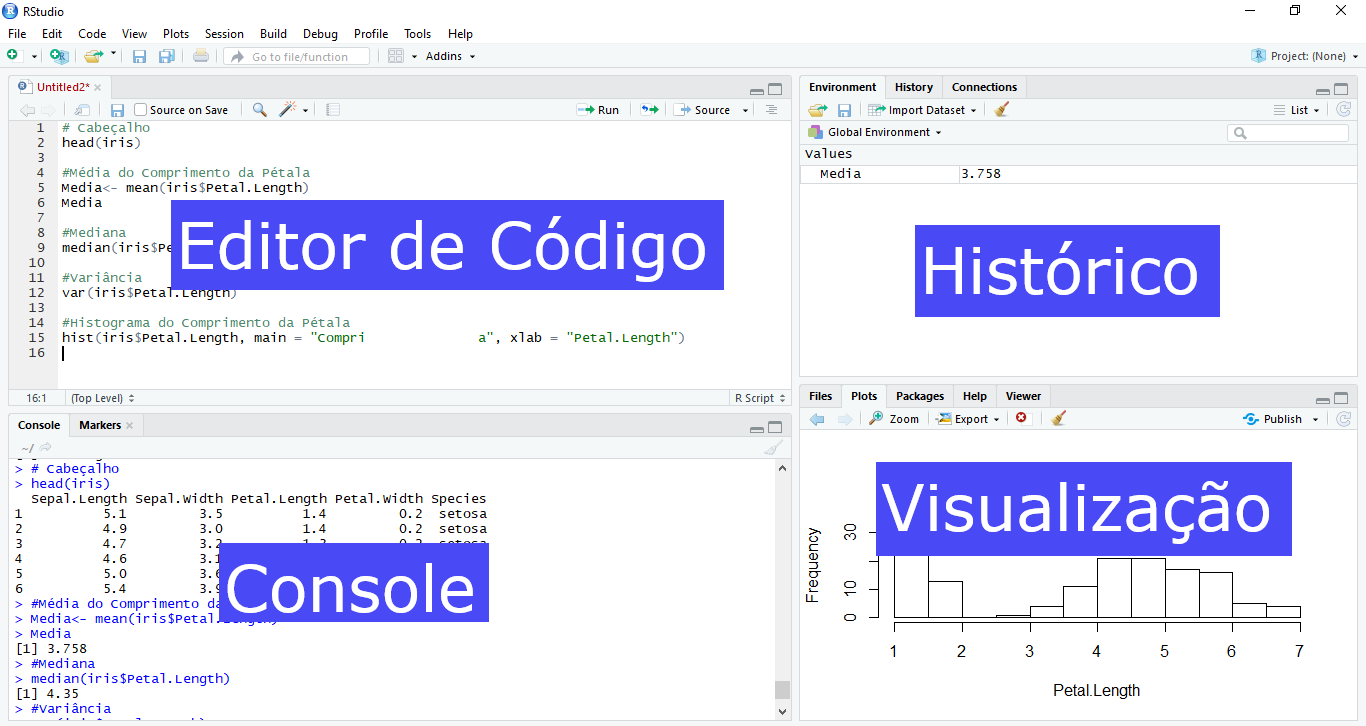
\includegraphics{figure/fig1_rstudio.png}
\caption{Janelas do RStudio. Ref: \url{https://www.est.ufmg.br/~cristianocs/Pacotes2021/Intro.html\#6}}
\end{figure}

\hypertarget{pacotes}{%
\section{Pacotes}\label{pacotes}}

Por ser \emph{Open Source}, o R permite que qualquer usuário disponibilize funções e bancos de dados a comunidade. As funções/bancos de dados são disponibilizados através de pacotes. A instalação de um pacote depende do repositório que ele está armazenado: máquina local, CRAN, GitHub, Bioconductor, entre outros. O repostitório CRAN contêm muitos pacotes e não é direcionado à uma área específica (como é o caso do Bioconductor que se destina a pacotes voltados para área de biotecnologia). A instalação de um pacote do repositório CRAN é feita pelo menu ``Tools \textgreater{} Install Packages'' ou simplesmente utilizando o seguinte comando:

\begin{Shaded}
\begin{Highlighting}[]
\FunctionTok{installed.packages}\NormalTok{(}\StringTok{"nomeDoPacote"}\NormalTok{)}
\end{Highlighting}
\end{Shaded}

Para que você possa utilizar as funções do pacote que instalou, você deve usar um dos dois comandos a seguir, para de fato carregar as funções do pacote para o ambiente R:

\begin{Shaded}
\begin{Highlighting}[]
\FunctionTok{library}\NormalTok{(nomeDoPacote)}
\FunctionTok{require}\NormalTok{(nomeDoPacote)}
\end{Highlighting}
\end{Shaded}

A função \texttt{library()} é utilizada normalmente no corpo do script, enquanto que a função \texttt{require()} é utilizada dentro de outras funções.

\hypertarget{comeuxe7ando-de-fato-a-programar-em-r}{%
\section{Começando de fato a programar em R}\label{comeuxe7ando-de-fato-a-programar-em-r}}

No console (janela do canto inferior esquerdo) digite o comando a seguir e tecle ENTER:

\begin{Shaded}
\begin{Highlighting}[]
\FunctionTok{print}\NormalTok{(}\StringTok{"Hello World"}\NormalTok{)}
\end{Highlighting}
\end{Shaded}

Agora digite o mesmo comando no editor de código (janela do canto superior esquerdo) e com o cursor na mesma linha do comando, tecle CTRL e ENTER simultaneamente:

\begin{Shaded}
\begin{Highlighting}[]
\FunctionTok{print}\NormalTok{(}\StringTok{"Hello World"}\NormalTok{)}
\end{Highlighting}
\end{Shaded}

A diferença é que quando executamos os comandos no editor de código, o comando continua no editor para ser executado, ou seja svocê está construindo um script. Mas você executa comando diretamente no console, eles não ficam gravados em um editor.

O dado de saída da função, foi um print do que estava dentro da função. Mas como você saber o que usar dentro de uma determinada função, como \texttt{print()}? Você precisa acessar o manual desta função.

\hypertarget{acessando-o-manual-da-funuxe7uxe3o}{%
\section{Acessando o manual da função}\label{acessando-o-manual-da-funuxe7uxe3o}}

Esta é uma etapa muito importante que antecede a sua caminhada no aprendizado do R. Você pode visualizar o manual da função executando um comando onde um ponto de interregoção (?) precisa anteceder a função:

\begin{Shaded}
\begin{Highlighting}[]
\NormalTok{?print}
\end{Highlighting}
\end{Shaded}

Mas se você deseja encontrar funções que realizam uma determinada ação, basta inserir dois pontos de interrogação antecedendo a ação desejada:

\begin{Shaded}
\begin{Highlighting}[]
\NormalTok{??priting}
\end{Highlighting}
\end{Shaded}

O comando acima realizará uma busca por tópicos que contenham a palavra \emph{ploting}. Outra opçõe alternativa ao \textbf{?} é o uso da função \texttt{help()} e \texttt{help.search()} para \textbf{??}

\begin{Shaded}
\begin{Highlighting}[]
\FunctionTok{help}\NormalTok{(}\StringTok{"print"}\NormalTok{)}
\FunctionTok{help.search}\NormalTok{(}\StringTok{"priting"}\NormalTok{)}
\end{Highlighting}
\end{Shaded}

Algumas funções possuem exemplos de sua execução. Se você quer saber como utilizar uma determinada função através de exemplos, execute a função \texttt{example()}.

\begin{Shaded}
\begin{Highlighting}[]
\FunctionTok{example}\NormalTok{(}\StringTok{"print"}\NormalTok{)}
\end{Highlighting}
\end{Shaded}

\hypertarget{comentando-cuxf3digos-no-r}{%
\section{Comentando códigos no R}\label{comentando-cuxf3digos-no-r}}

A maioria das linguagens de programação e até linguagem de marcação, possuem uma forma de inserção de textos que não serão executados pela linguagem. Esse procedimento é denominado de comentário. Você pode comentar os seus códigos. Isso é algo essencial para todos os programadores, indiferente da linguagem. Pois, códigos comentados facilitam a interpretação do mesmo por outros programadores e até mesmo pelo autor, devido a um período de tempo que se passou desde a criação daquele código.

Para comentar linhas no R você precisa inserir o \texttt{\#} antes do que seria o comentário:

\begin{Shaded}
\begin{Highlighting}[]
\CommentTok{\# isto é um comentário}
\end{Highlighting}
\end{Shaded}

Exemplo aplicado:

\begin{Shaded}
\begin{Highlighting}[]
\FunctionTok{print}\NormalTok{(}\StringTok{"Hello World"}\NormalTok{) }\CommentTok{\# imprimindo na tela Hello World}
\end{Highlighting}
\end{Shaded}

Perceba que o conteúdo após o \texttt{\#} não é interpretado no R, ou seja, este conteúdo é um comentário.

\hypertarget{cross}{%
\chapter{Cross-references}\label{cross}}

Cross-references make it easier for your readers to find and link to elements in your book.

\hypertarget{chapters-and-sub-chapters}{%
\section{Chapters and sub-chapters}\label{chapters-and-sub-chapters}}

There are two steps to cross-reference any heading:

\begin{enumerate}
\def\labelenumi{\arabic{enumi}.}
\tightlist
\item
  Label the heading: \texttt{\#\ Hello\ world\ \{\#nice-label\}}.

  \begin{itemize}
  \tightlist
  \item
    Leave the label off if you like the automated heading generated based on your heading title: for example, \texttt{\#\ Hello\ world} = \texttt{\#\ Hello\ world\ \{\#hello-world\}}.
  \item
    To label an un-numbered heading, use: \texttt{\#\ Hello\ world\ \{-\#nice-label\}} or \texttt{\{\#\ Hello\ world\ .unnumbered\}}.
  \end{itemize}
\item
  Next, reference the labeled heading anywhere in the text using \texttt{\textbackslash{}@ref(nice-label)}; for example, please see Chapter \ref{cross}.

  \begin{itemize}
  \tightlist
  \item
    If you prefer text as the link instead of a numbered reference use: \protect\hyperlink{cross}{any text you want can go here}.
  \end{itemize}
\end{enumerate}

\hypertarget{captioned-figures-and-tables}{%
\section{Captioned figures and tables}\label{captioned-figures-and-tables}}

Figures and tables \emph{with captions} can also be cross-referenced from elsewhere in your book using \texttt{\textbackslash{}@ref(fig:chunk-label)} and \texttt{\textbackslash{}@ref(tab:chunk-label)}, respectively.

See Figure \ref{fig:nice-fig}.

\begin{Shaded}
\begin{Highlighting}[]
\FunctionTok{par}\NormalTok{(}\AttributeTok{mar =} \FunctionTok{c}\NormalTok{(}\DecValTok{4}\NormalTok{, }\DecValTok{4}\NormalTok{, .}\DecValTok{1}\NormalTok{, .}\DecValTok{1}\NormalTok{))}
\FunctionTok{plot}\NormalTok{(pressure, }\AttributeTok{type =} \StringTok{\textquotesingle{}b\textquotesingle{}}\NormalTok{, }\AttributeTok{pch =} \DecValTok{19}\NormalTok{)}
\end{Highlighting}
\end{Shaded}

\begin{figure}

{\centering 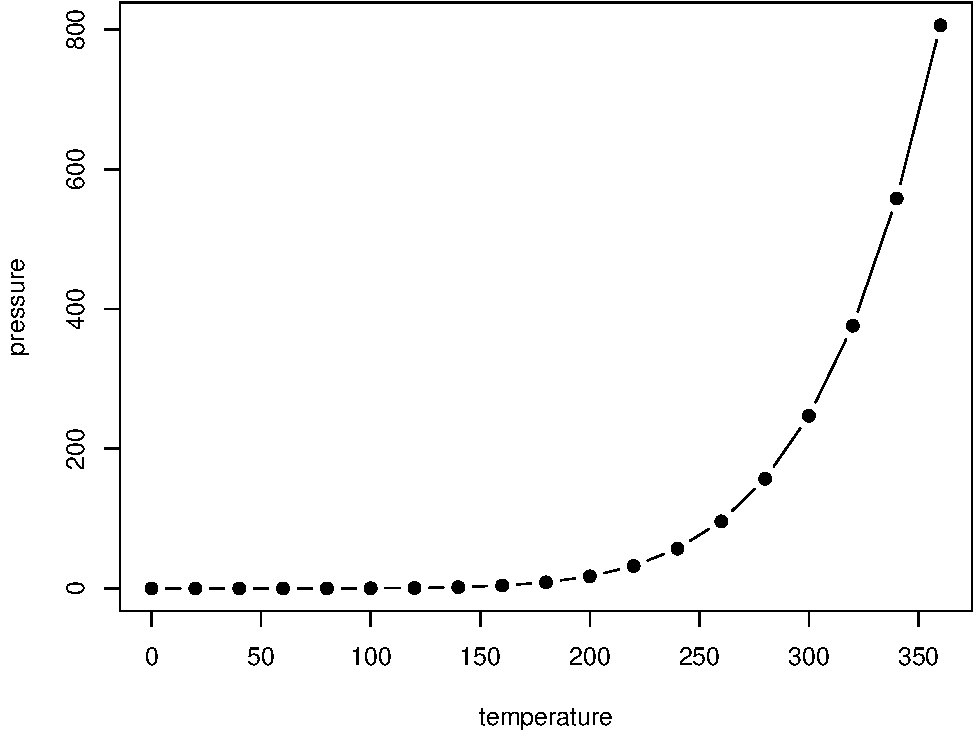
\includegraphics[width=0.8\linewidth]{_main_files/figure-latex/nice-fig-1} 

}

\caption{Here is a nice figure!}\label{fig:nice-fig}
\end{figure}

Don't miss Table \ref{tab:nice-tab}.

\begin{Shaded}
\begin{Highlighting}[]
\NormalTok{knitr}\SpecialCharTok{::}\FunctionTok{kable}\NormalTok{(}
  \FunctionTok{head}\NormalTok{(pressure, }\DecValTok{10}\NormalTok{), }\AttributeTok{caption =} \StringTok{\textquotesingle{}Here is a nice table!\textquotesingle{}}\NormalTok{,}
  \AttributeTok{booktabs =} \ConstantTok{TRUE}
\NormalTok{)}
\end{Highlighting}
\end{Shaded}

\begin{table}

\caption{\label{tab:nice-tab}Here is a nice table!}
\centering
\begin{tabular}[t]{rr}
\toprule
temperature & pressure\\
\midrule
0 & 0.0002\\
20 & 0.0012\\
40 & 0.0060\\
60 & 0.0300\\
80 & 0.0900\\
\addlinespace
100 & 0.2700\\
120 & 0.7500\\
140 & 1.8500\\
160 & 4.2000\\
180 & 8.8000\\
\bottomrule
\end{tabular}
\end{table}

\hypertarget{parts}{%
\chapter{Parts}\label{parts}}

You can add parts to organize one or more book chapters together. Parts can be inserted at the top of an .Rmd file, before the first-level chapter heading in that same file.

Add a numbered part: \texttt{\#\ (PART)\ Act\ one\ \{-\}} (followed by \texttt{\#\ A\ chapter})

Add an unnumbered part: \texttt{\#\ (PART\textbackslash{}*)\ Act\ one\ \{-\}} (followed by \texttt{\#\ A\ chapter})

Add an appendix as a special kind of un-numbered part: \texttt{\#\ (APPENDIX)\ Other\ stuff\ \{-\}} (followed by \texttt{\#\ A\ chapter}). Chapters in an appendix are prepended with letters instead of numbers.

\hypertarget{footnotes-and-citations}{%
\chapter{Footnotes and citations}\label{footnotes-and-citations}}

\hypertarget{footnotes}{%
\section{Footnotes}\label{footnotes}}

Footnotes are put inside the square brackets after a caret \texttt{\^{}{[}{]}}. Like this one \footnote{This is a footnote.}.

\hypertarget{citations}{%
\section{Citations}\label{citations}}

Reference items in your bibliography file(s) using \texttt{@key}.

For example, we are using the \textbf{bookdown} package \citep{R-bookdown} (check out the last code chunk in index.Rmd to see how this citation key was added) in this sample book, which was built on top of R Markdown and \textbf{knitr} \citep{xie2015} (this citation was added manually in an external file book.bib).
Note that the \texttt{.bib} files need to be listed in the index.Rmd with the YAML \texttt{bibliography} key.

The RStudio Visual Markdown Editor can also make it easier to insert citations: \url{https://rstudio.github.io/visual-markdown-editing/\#/citations}

\hypertarget{blocks}{%
\chapter{Blocks}\label{blocks}}

\hypertarget{equations}{%
\section{Equations}\label{equations}}

Here is an equation.

\begin{equation} 
  f\left(k\right) = \binom{n}{k} p^k\left(1-p\right)^{n-k}
  \label{eq:binom}
\end{equation}

You may refer to using \texttt{\textbackslash{}@ref(eq:binom)}, like see Equation \eqref{eq:binom}.

\hypertarget{theorems-and-proofs}{%
\section{Theorems and proofs}\label{theorems-and-proofs}}

Labeled theorems can be referenced in text using \texttt{\textbackslash{}@ref(thm:tri)}, for example, check out this smart theorem \ref{thm:tri}.

\begin{theorem}
\protect\hypertarget{thm:tri}{}\label{thm:tri}For a right triangle, if \(c\) denotes the \emph{length} of the hypotenuse
and \(a\) and \(b\) denote the lengths of the \textbf{other} two sides, we have
\[a^2 + b^2 = c^2\]
\end{theorem}

Read more here \url{https://bookdown.org/yihui/bookdown/markdown-extensions-by-bookdown.html}.

\hypertarget{callout-blocks}{%
\section{Callout blocks}\label{callout-blocks}}

The R Markdown Cookbook provides more help on how to use custom blocks to design your own callouts: \url{https://bookdown.org/yihui/rmarkdown-cookbook/custom-blocks.html}

\hypertarget{sharing-your-book}{%
\chapter{Sharing your book}\label{sharing-your-book}}

\hypertarget{publishing}{%
\section{Publishing}\label{publishing}}

HTML books can be published online, see: \url{https://bookdown.org/yihui/bookdown/publishing.html}

\hypertarget{pages}{%
\section{404 pages}\label{pages}}

By default, users will be directed to a 404 page if they try to access a webpage that cannot be found. If you'd like to customize your 404 page instead of using the default, you may add either a \texttt{\_404.Rmd} or \texttt{\_404.md} file to your project root and use code and/or Markdown syntax.

\hypertarget{metadata-for-sharing}{%
\section{Metadata for sharing}\label{metadata-for-sharing}}

Bookdown HTML books will provide HTML metadata for social sharing on platforms like Twitter, Facebook, and LinkedIn, using information you provide in the \texttt{index.Rmd} YAML. To setup, set the \texttt{url} for your book and the path to your \texttt{cover-image} file. Your book's \texttt{title} and \texttt{description} are also used.

This \texttt{gitbook} uses the same social sharing data across all chapters in your book- all links shared will look the same.

Specify your book's source repository on GitHub using the \texttt{edit} key under the configuration options in the \texttt{\_output.yml} file, which allows users to suggest an edit by linking to a chapter's source file.

Read more about the features of this output format here:

\url{https://pkgs.rstudio.com/bookdown/reference/gitbook.html}

Or use:

\begin{Shaded}
\begin{Highlighting}[]
\NormalTok{?bookdown}\SpecialCharTok{::}\NormalTok{gitbook}
\end{Highlighting}
\end{Shaded}


  \bibliography{book.bib,packages.bib}

\end{document}
